\documentclass{article}
\usepackage{graphicx}
\usepackage{tikz}


\title{Final project}

\date{4031}

\author{Ehsan Esmaeili}

\begin{document}


\maketitle
\newpage

\tableofcontents

\newpage

\section{GIT AND GITHUB}

\subsection{Repository Initialization and Commits}
\begin{itemize}
   

 \item crate a repasitory

 \item clone it with (git clone url)

 \item make a file (main.tex)

 \item change file and use these command:

  git add .

  git commit -m (Initialize LaTeX document)

  git push origin main
\end{itemize}
\subsection{GitHub Actions for LaTeX Compilation}

\begin{itemize}

\item crate a file ------.yml in the workflows in the .GitHub

\item past main.yml from miliaxe project

\item when you insert tag workflows goes to running
\end{itemize}
\newpage

\section{EXPLORATION TASKS}

\subsection{Vim Advanced Features}
\begin{itemize}

\item Macros: Record and replay repetitive commands. 

\item Regex search: Search patterns using regular expressions.

\item Multiple edits: Edit multiple files simultaneously with :argdo.
\end{itemize}
\subsection{Memory profiling}

Occurs when allocated memory is not released, leading to performance degradation.

Valgrind is a powerful open-source framework for debugging, profiling, 
and analyzing programs, primarily focused on memory management and performance. 
It runs programs in a virtual machine-like environment, allowing it to closely monitor their behavior.

\subsection{GNU/Linux Bash Scripting}


Fuzzy searching: Finding approximate matches for user input.

Command ls | fzf: Lists files and lets you select one.
\begin{itemize}

\item fd -e pdf 

\item fd -e pdf | fzf  

\item zathura \$(fd -e pdf | fzf)
  \end{itemize}
\newpage

\section{GIT AND FOSS}

\subsection{README.md}

Included a simple README.md with repository objectives.

\subsection{Issues}

\begin{figure}[h]
    \centering
    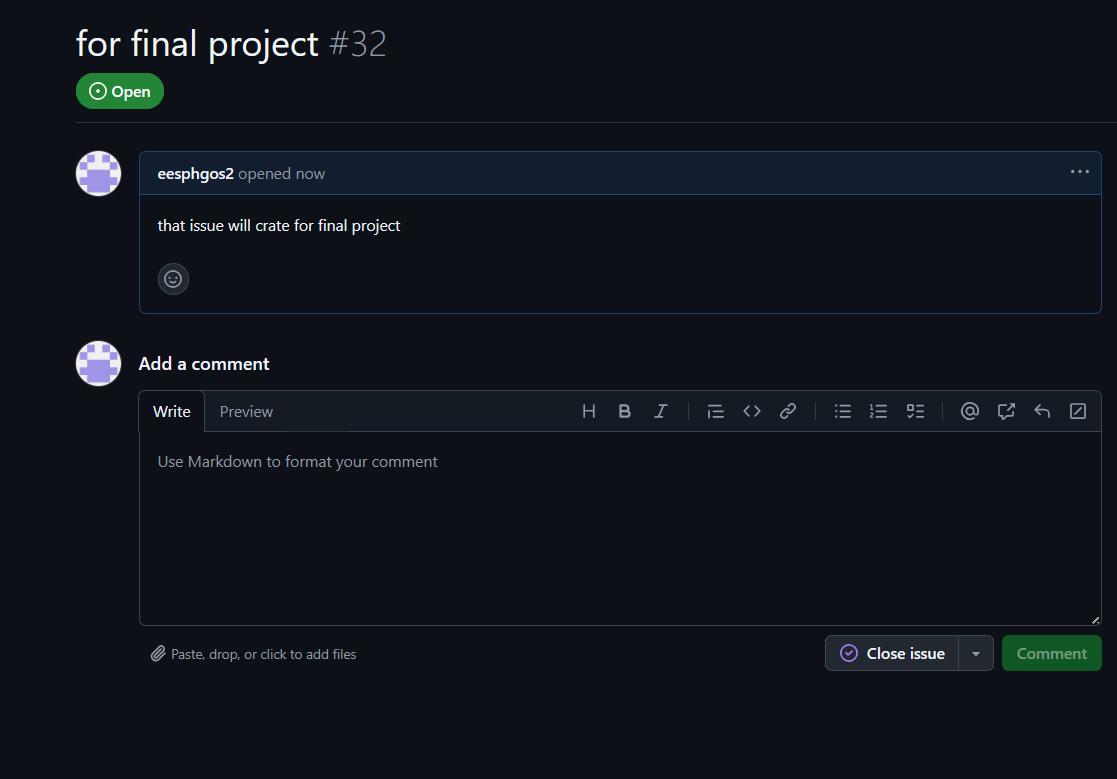
\includegraphics[width=1\linewidth]{Screenshot 2025-01-20 092658}
    \*{issue}
\end{figure}

\subsection{FOSS contribution}

Yes, I’m interested in contributing to tools for developers and open-source gaming projects.

the foss contributing can delop skills experiencly.


\end{document}
